\documentclass[varwidth=false, border=2pt]{standalone}

\usepackage{pgfplots}
\usepackage{tikz}
\usepackage{nicefrac}
\pgfplotsset{every axis legend/.append style={
at={(0,0)},
anchor=north east}}

\begin{document}
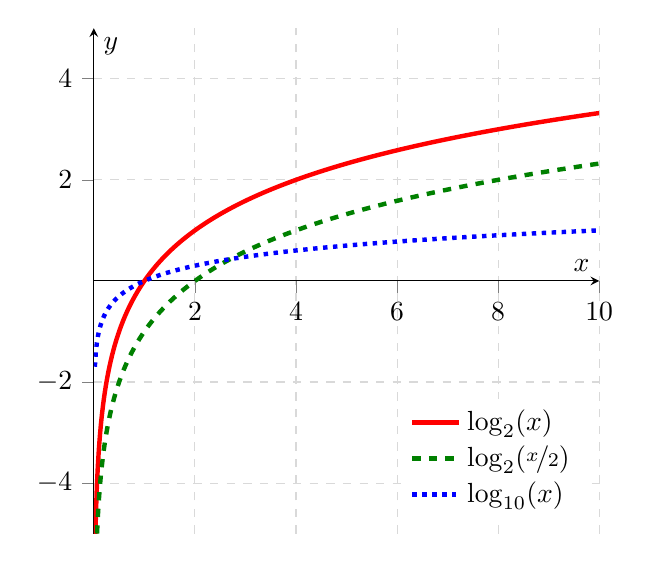
\begin{tikzpicture}
    \begin{axis}[
        axis x line=middle,
        axis y line=middle,
        grid = major,
        width=8cm,
        height=8cm,
        grid style={dashed, gray!30},
        xmin= 0,   % start the diagram at this x-coordinate
        xmax=10,   % end   the diagram at this x-coordinate
        ymin=-5,   % start the diagram at this y-coordinate
        ymax= 5,   % end   the diagram at this y-coordinate
        xlabel=$x$,
        ylabel=$y$,
        legend cell align=left,
        legend pos=south east,
        legend style={draw=none},
        tick align=outside,
        enlargelimits=false]
      % plot the function
      \addplot[domain=0:10, red, ultra thick,samples=500] {log2(x)};
      \addplot[domain=0:10, green!50!black,dashed,ultra thick,samples=500] {log2(0.5*x)};
      \addplot[domain=0:10, blue,dotted, ultra thick,samples=500] {log10(x)};
      \legend{$\log_2(x)$,$\log_2(\nicefrac{x}{2})$,$\log_{10}(x)$}
    \end{axis}
\end{tikzpicture}
\end{document}
